\documentclass[12pt]{article}
\usepackage{graphicx}
%\documentclass[journal,12pt,twocolumn]{IEEEtran}
\usepackage[none]{hyphenat}
\usepackage{gensymb}
\usepackage{commath}
\usepackage{listings}
\usepackage[english]{babel}
\usepackage{caption}
\usepackage{amssymb}
\usepackage{hyperref}
\usepackage{enumitem}
\usepackage{booktabs}
\usepackage{array}
\usepackage{amsmath}   % for having text in math mode
\usepackage{listings}
\lstset{
  frame=single,
  breaklines=true
}
%New macro definitions
\newcommand{\mydet}[1]{\ensuremath{\begin{vmatrix}#1\end{vmatrix}}}
\providecommand{\brak}[1]{\ensuremath{\left(#1\right)}}
\providecommand{\norm}[1]{\left\lVert#1\right\rVert}
\newcommand{\solution}{\noindent \textbf{Solution: }}
\newcommand{\myvec}[1]{\ensuremath{\begin{pmatrix}#1\end{pmatrix}}}
\let\vec\mathbf


\begin{document}
\begin{center}
\textbf\large{CLASS-9\\CHAPTER-10 \\ CIRCLES}
\end{center}
\section*{Exercise 10.4}
\begin{enumerate}
\item If two equal chords of a circle intersect prove that the parts of one chord are separately equal to the parts of the other chord
\item If non-parallel sides of a trapezium are equal. prove that it is cyclic
\item If $\vec{P},\vec{Q}$ and $\vec{R}$ are the mid-points of the sides $BC$, $CA$ and $AB$ of a triangle and $AD$ is the perpendicular from $A$ on $BC$, prove that $\vec{P},\vec{Q},\vec{R}$ and $\vec{D}$ are concyclic
\item $ABCD$ is a parallelogram. A circle through $\vec{A}$, $\vec{B}$ is so drawn that it intersects $AD$ at $\vec{P}$ and $BC$ at $\vec{Q}$. prove that $\vec{P}$, $\vec{Q}$, $\vec{R}$ and $\vec{D}$ are concyclic.
\item Prove that angle bisector of any angle of a triangle and perpendicular bisector of the opposite side if intersect, they will intersent on the circumcircle of the triangle.
\item If two chords $AB$ and $CD$ of a circle AYDZBWCX intersect at right angles see Fig \ref{fig:1}, prove that
	\begin{align}
		arc\brak{CXA}+arc\brak{DZB}=arc\brak{AYD}+arc\brak{AYD}+arc\brak{BWC}= semi-circle
	\end{align}
	\begin{figure}[h!]                        \begin{center}                                   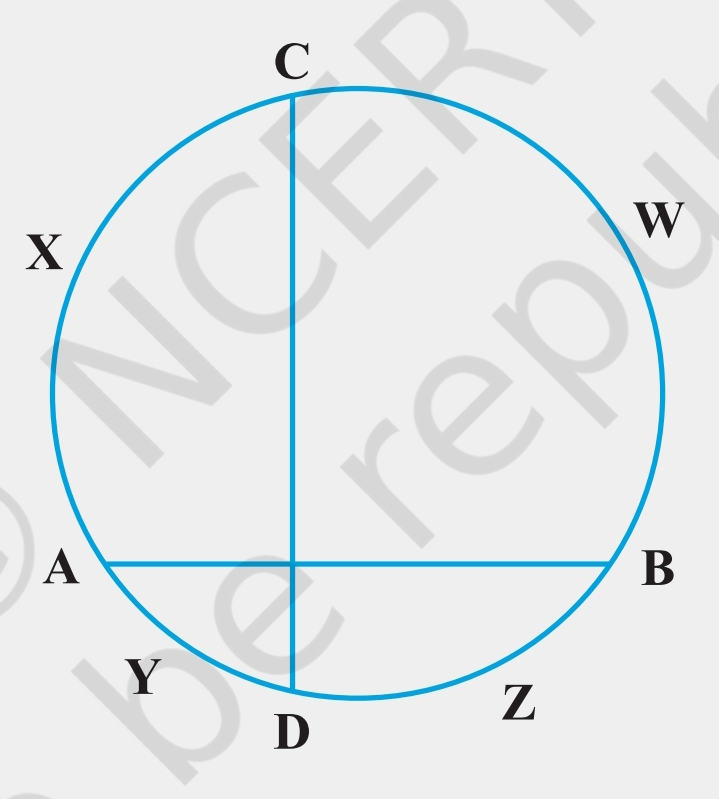
\includegraphics[width=\columnwidth]{image1.jpg}                          \end{center}                            \caption{}                                       \label{fig:1}                    \end{figure}
	\item If $ABC$ is an equilateral triangle inscribed in a circle and $\vec{P}$ be any point on the minor arc $BC$ which does nat coincide with $\vec{B}$ or $\vec{C}$, prove that $PA$ is angle bisector of $\angle BPC$
	\item In Fig-\ref{fig:2}, $AB$ and $CD$ are two chords of a circle intersecting each other at point $\vec{E}$ prove that $\angle AEC=\frac{1}{2}$ $c$ Angle subtended by arc $CXA$ at centre + angle subtended by arc $DY$ $B$ at the centre).
	\begin{figure}[h!]                        \begin{center}                                   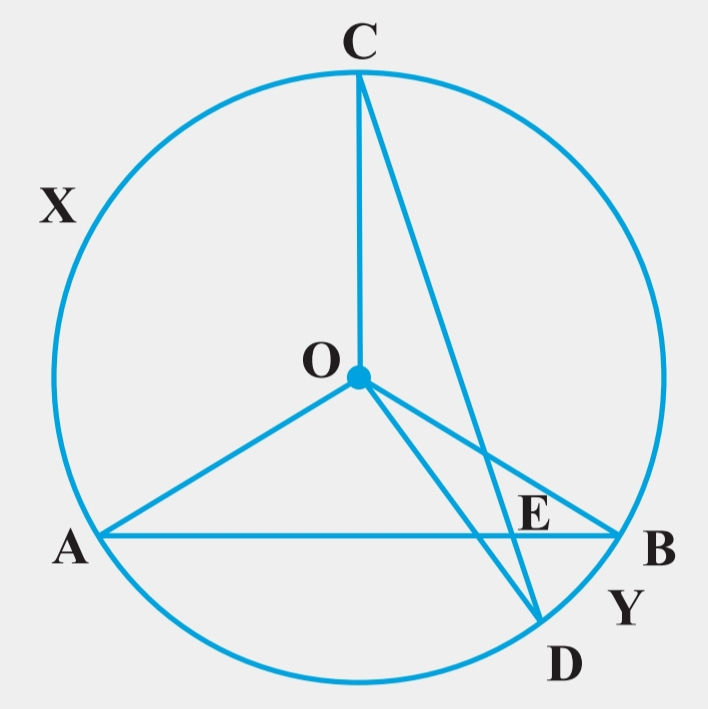
\includegraphics[width=\columnwidth]{image2.jpg}                          \end{center}                            \caption{}                                       \label{fig:2}                    \end{figure}
	\item If bisectors of opposite angles of a cyclic quadrilateral $ABCD$ intersect the circle, circumscribing it at the points $\vec{P}$ and $\vec{Q}$, prove that $PQ$ is a diameter of the circle,
\item A circle has radius $\sqrt{442}$ cm it is divided into two segments by a chord of length 2cm. prove that the angle subtended by the chord at a point in major segment is $45\degree$.
\item Two equal chords $AB$ and $CD$ of a circle when produced intersect at a point $\vec{P}$ prove that $PB=PD$
\item $AB$ and $AC$ are two chords of a circle of radius r such that $AB=2AC$. If $\vec{P}$ and $\vec{Q}$ are the distances of $AB$ and $AC$ from the centre, prove that $4q^2=p^2+3r^2$
\item In Fig \ref{fig:3}, $\vec{O}$ is the centre of the circle, $\angle BCO=30\degree$.Find $x$ and $y$
	\begin{figure}[h!]                        \begin{center}                                   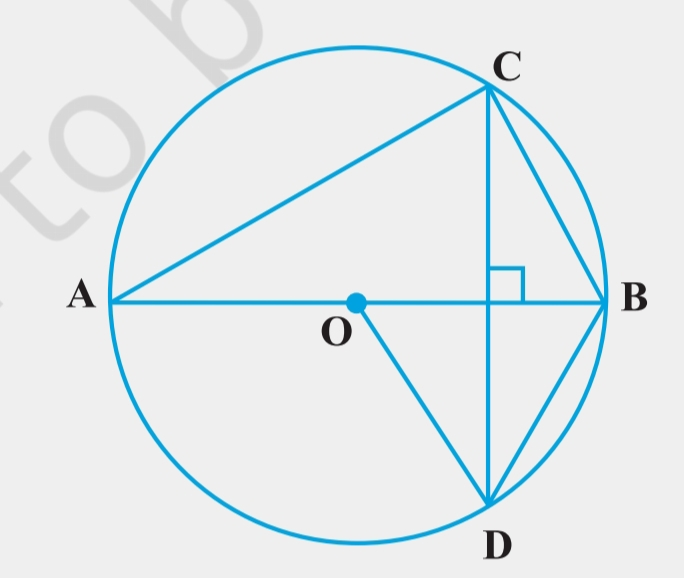
\includegraphics[width=\columnwidth]{image3.jpg}                          \end{center}                            \caption{}                                       \label{fig:3}                    \end{figure}
	\item In fig \ref{fig:4}, $\vec{O}$ is the centre of the circle $BD=0D$ and $CD \bot AB$. Find $\angle CAB$
	\begin{figure}[h!]                        \begin{center}                                   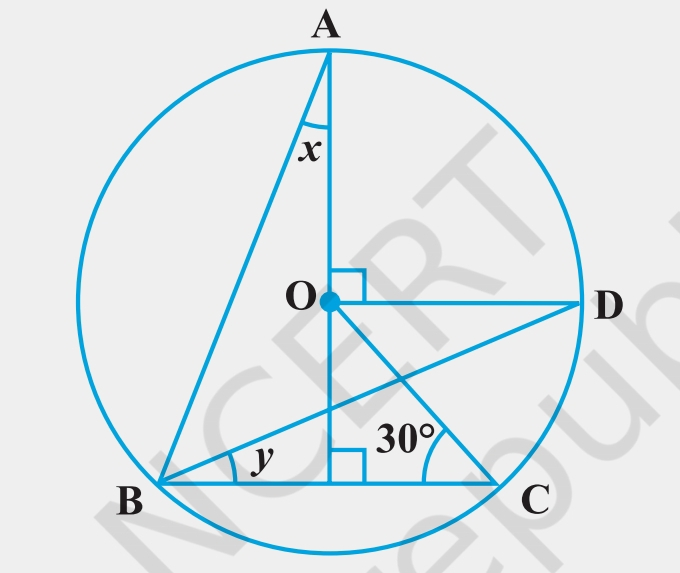
\includegraphics[width=\columnwidth]{image4.jpg}                          \end{center}                            \caption{}                                       \label{fig:4}                    \end{figure}
\end{enumerate}

	
\end{document}
